\chapter{Mecánica de Fluidos}
\noindent

\section{Introducción}

El cálculo de variaciones visto en Modelos Matemáticos II se consideraba ``matemática pura''. Pasó de los matemáticos puros, al ámbito 
de los físicos. Ahora en física hay algo en cuarto de mecánica analítica (que es fácil para ellos). Los ingenieros están usando también
la mecánica, y ahora está volviendo a la matemática. \\

El primero fue Euler. Lo que vamos a ver ahora son las ecuaciones de Euler. En París a principios del siglo XIX. Había que canalizar el agua,
ver cómo se podía distribuir. El surgimiento vino con Navier y Stokes. La mecánica de fluidos ha quedado en manos de las matemáticas. Veremos 
tres o cuatro corrientes que surgen de la mecánica de fluidos. \\

Los únicos que le dedican un poco de atención son los ingenieros aeronáuticos. Los que diseñan el coche de Fernando Alonso que se están equivocando. 
Detrás del diseño de los coches y aviones, en general están matemáticos. \\

Otro lugar en el que los fluidos son importantes es en el ámbito del clima. Hoy en día se predice 2 o 3 días antes. Empiezan diciendo, según
nuestros modelos (los modelos son los mismos), lo que cambia es cómo se resuelve el modelo, y cómo resuelve Navier-Stokes. Hay modelos que 
consideran la orografía, pero, en general, cuanto más realista es el modelo, más complicado es de resolver. \\

Vamos a comenzar por el caso $2$-dimensional, y con las ecuaciones de Euler. Tenemos un plano y se trata de describir cómo se mueve un fluido.
Gráficamente:
\begin{figure}[H]
    \begin{center}
        \tikzset{every picture/.style={line width=0.75pt}} %set default line width to 0.75pt        
            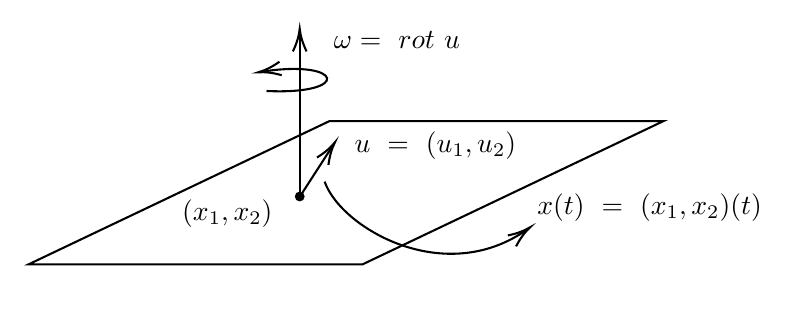
\begin{tikzpicture}[x=0.75pt,y=0.75pt,yscale=-1,xscale=1]
            %uncomment if require: \path (0,300); %set diagram left start at 0, and has height of 300

            %Shape: Rectangle [id:dp7209051313285793] 
            \draw   (294.35,76.5) -- (455.26,76.5) -- (310.34,145.5) -- (149.43,145.5) -- cycle ;
            %Straight Lines [id:da648079438822599] 
            \draw    (280,111) -- (280,34) ;
            \draw [shift={(280,32)}, rotate = 90] [color={rgb, 255:red, 0; green, 0; blue, 0 }  ][line width=0.75]    (10.93,-3.29) .. controls (6.95,-1.4) and (3.31,-0.3) .. (0,0) .. controls (3.31,0.3) and (6.95,1.4) .. (10.93,3.29)   ;
            %Curve Lines [id:da02355300563515772] 
            \draw    (264,62) .. controls (305.37,63.97) and (301.14,46.54) .. (261.82,52.7) ;
            \draw [shift={(260,53)}, rotate = 350.31] [color={rgb, 255:red, 0; green, 0; blue, 0 }  ][line width=0.75]    (10.93,-3.29) .. controls (6.95,-1.4) and (3.31,-0.3) .. (0,0) .. controls (3.31,0.3) and (6.95,1.4) .. (10.93,3.29)   ;
            %Shape: Circle [id:dp28371925872083015] 
            \draw  [color={rgb, 255:red, 0; green, 0; blue, 0 }  ,draw opacity=1 ][fill={rgb, 255:red, 0; green, 0; blue, 0 }  ,fill opacity=1 ] (281.83,112.83) .. controls (281.83,111.82) and (281.01,111) .. (280,111) .. controls (278.99,111) and (278.17,111.82) .. (278.17,112.83) .. controls (278.17,113.85) and (278.99,114.67) .. (280,114.67) .. controls (281.01,114.67) and (281.83,113.85) .. (281.83,112.83) -- cycle ;
            %Straight Lines [id:da556275463205884] 
            \draw    (280,113) -- (295.92,88.35) ;
            \draw [shift={(297,86.67)}, rotate = 122.85] [color={rgb, 255:red, 0; green, 0; blue, 0 }  ][line width=0.75]    (10.93,-3.29) .. controls (6.95,-1.4) and (3.31,-0.3) .. (0,0) .. controls (3.31,0.3) and (6.95,1.4) .. (10.93,3.29)   ;
            %Curve Lines [id:da8523005951397323] 
            \draw    (292,105.67) .. controls (299.92,128.11) and (349.98,157.08) .. (389.8,128.55) ;
            \draw [shift={(391,127.67)}, rotate = 143.13] [color={rgb, 255:red, 0; green, 0; blue, 0 }  ][line width=0.75]    (10.93,-3.29) .. controls (6.95,-1.4) and (3.31,-0.3) .. (0,0) .. controls (3.31,0.3) and (6.95,1.4) .. (10.93,3.29)   ;

            % Text Node
            \draw (295,32) node [anchor=north west][inner sep=0.75pt]   [align=left] {$\displaystyle \omega =\ \text{rot} \ u$};
            % Text Node
            \draw (221.89,113) node [anchor=north west][inner sep=0.75pt]   [align=left] {$\displaystyle ( x_{1} ,x_{2})$};
            % Text Node
            \draw (305,80) node [anchor=north west][inner sep=0.75pt]   [align=left] {$\displaystyle u\ =\ ( u_{1} ,u_{2})$};
            % Text Node
            \draw (393,110) node [anchor=north west][inner sep=0.75pt]   [align=left] {$\displaystyle x( t) \ =\ ( x_{1} ,x_{2})( t)$};
        \end{tikzpicture}
    \end{center}
\end{figure}
Ya vimos en \ref{section:rot} la definición del rotacional, en inglés \textit{curl}. Cada punto está afectado por una presión. Se trata de ver cuáles son las ecuaciones que verifican el modelo anterior.
Consideramos\footnote{A priori no sabemos si será $[0,T]$.}
\begin{equation}\label{eq:ec24}
    u : \left[0, T \right[ \times \R^2 \to \R^2
\end{equation}
    
y la ecuación 

\begin{equation}\label{eq:ec22}
    \dfrac{\partial u}{\partial t} + (u \cdot \nabla) u + \nabla p = 0
\end{equation}
¿Qué significa \eqref{eq:ec22}? Analizamos sumando a sumando:
\begin{itemize}
    \item En primer lugar, $$u \cdot \nabla = \sum_{j=1}^{2} u_j \dfrac{\partial}{\partial x_j}$$
    \item Como $p$ es un escalar $$\nabla p = \left( \dfrac{\partial p}{\partial x_1}, \dfrac{\partial p}{\partial x_2} \right)$$ 
\end{itemize}

Hay muchos tipos de fluido. El aire que tenemos aquí es un fluido. Si tuviéramos una jeringa, podríamos comprimir el aire. Nosotros vamos a 
suponer ahora que estudiamos fluidos incompresibles, es decir, $\di(u) = 0$, donde
$$\di(u) = \dfrac{\partial u_1}{\partial x_1} + \dfrac{\partial u_2}{\partial x_2}$$
Vemos ahora que a $u$ se le asocia la ecuación
$$\dfrac{\partial u}{\partial t} + (a \cdot \nabla) u = 0$$
$$\dfrac{\partial X}{\partial t} = \di(a)$$
Vemos que en lugar de $u \cdot \nabla$ ponemos $a \cdot \nabla$. \\

Una condición natural es que $|u(t,x)| \to 0$ cuando $|x| \to \infty$. Ahora nos preguntamos qué pasa en el tiempo inicial, para lo cual
tendremos en cuenta una condición inicial: $u(t=0,x) = u_0(x)$. Recopilando todo:

\begin{definicion}[Ecuaciones de Euler]
    Las ecuaciones de Euler en $\R^N$, con $N=2,3$, son:
    \begin{equation}\label{eq:ec23}
        \begin{cases}
            \dfrac{\partial u}{\partial t} + (u \cdot \nabla) u + \nabla p = 0 \\
            \di(u) = 0 \\
            |u(t,x)| \to 0 \quad |x| \to +\infty \\
            u(t=0,x) = u_0(x)
        \end{cases}
    \end{equation}
\end{definicion}

\begin{observacion}
    Vemos que las ecuaciones son las mismas tanto para $N=2$ como para $N=3$. Para $N=4$ puede tener sentido, por ejemplo, en el ámbito de la gravitación.
    En el caso bidimensional, podemos tomar componentes en la primera ecuación de \eqref{eq:ec23}, y obtener
    \begin{equation}
        \dfrac{\partial u_i}{\partial t} + (u \cdot \nabla) u_i + \dfrac{\partial p}{\partial x_i} = 0 \quad i=1,2
    \end{equation}
\end{observacion}

Otro vector importante a tener en cuenta es el vector vorticidad $\omega$. ¿Por qué? Porque muchas veces lo que es importante del fluido 
no es la velocidad en sí, o la presión, sino cuándo hay una turbulencia (rotación con mucha fuerza), y esto último se puede medir bien en los 
mapas del tiempo. \\

¿Qué es la vorticidad?:

\begin{definicion}[Vorticidad]
    Definimos $\omega$ como el rotacional del vector de velocidades $u$. Es decir
    $$\omega = \rot(u)$$
    donde\footnote{Consultar \ref{section:rot} si se quiere recordar más en profundidad.} 
    $$\rot(u) = \nabla \times u = \begin{vmatrix}
        i & \frac{\partial}{\partial x_1} & u_1(t, x_1, x_2) \\\\
        j & \frac{\partial}{\partial x_2} & u_2(t, x_1, x_2) \\\\
        k & \frac{\partial}{\partial x_3} & u_3(t, x_1, x_2)
    \end{vmatrix} = \left(0, 0, \overbrace{\dfrac{\partial u_2}{\partial x_1} - \dfrac{\partial u_1}{\partial x_2}}^{\omega} \right)$$
\end{definicion}

\begin{observacion}
    No tiene sentido, a priori, definirlo fuera de $\R^3$.
\end{observacion}

\begin{ejercicio} % TODO: Hacer para mañana
    Comprobar que la siguiente expresión es cierta:
    $$\rot((u \cdot \nabla)u) = (u \cdot \nabla) \omega + \di(u) \omega$$
    Podemos hacerlo componente a componente y sumar o como sea. \\

    Como el fluido es incompresible, $\di(u) \omega = 0$, y se simplifica la expresión anterior.
\end{ejercicio}

Otra pregunta es si podemos aplicar el rotacional de la primera ecuación de \eqref{eq:ec23}. Pues a priori no, pero vamos a hacerlo,
y luego analizamos cuándo tiene sentido esta expresión. \\

\begin{equation}
    \dfrac{\partial \omega}{\partial t} + (u \cdot \nabla) \omega + \rot(\nabla p) = 0
\end{equation}

\begin{observacion}
    En dimensión 3 aparece el siguiente término:
    $$(u \cdot \nabla) \omega - \boxed{(\omega \cdot \nabla) u} \di(u) \omega$$
    Este sustraendo señalado es el que representa la \textit{deformación de la vorticidad}, y es el culpable de muchas cosas que pasan
    en el caso tridimensional que en el bidimensional no ocurren (por ejemplo, el estudio de la regularidad de $\omega$).
\end{observacion}

Veamos cuánto vale $\rot(\nabla p)$: 

$$\rot(\nabla p) = \dfrac{\partial \dfrac{\partial p}{\partial x_2}}{\partial x_1} - \dfrac{\partial \dfrac{\partial p}{\partial x_1}}{\partial x_2} = 0$$

Por lo tanto tenemos hasta el momento la siguiente ecuación:

\begin{equation}\label{eq:ec25}
    \dfrac{\partial \omega}{\partial t} + (u \cdot \nabla) \omega = 0
\end{equation}

Siguen siendo tres incógnitas, pero hemos pasado de una ecuación vectorial a escalar ($\omega$ es el escalar). Otras ecuaciones que debemos considerar son
$$\omega = \rot(u)$$
$$\di(u) = 0$$
$$|u| \to 0 \quad |x| \to 0$$
$$\omega(t=0,x) = \omega_0(x)$$

No hemos simplificado gran cosa hasta ahora, pero nos disponemos a hacerlo. \\

Usaremos el siguiente lema de Poincaré:

\begin{lema}[de Poincaré]
    Sea $u$ un campo de velocidades en $\R^2$ como \eqref{eq:ec24}. Entonces se tiene que 
    $$\di(u) = 0 \iff \exists \psi : u = \rot(\psi)$$
\end{lema}

\begin{observacion}
    Para una formulación más técnica habría que estudiar $1$-formas (cosa que no vamos a hacer). La implicación hacia la derecha es sencilla,
    ya que basta aplicar rotacional. Así:
    $$\rot(\psi) = \left(
        \dfrac{\partial \psi}{\partial x_2}, - \dfrac{\partial \psi}{\partial x_1}, 0
    \right)$$
    Como $$\di\left( \dfrac{\partial \psi}{\partial x_2}, - \dfrac{\partial \psi}{\partial x_1} \right) = 
    \dfrac{\partial}{\partial x_1} \left( \dfrac{\partial \psi}{\partial x_2} \right) + 
    \dfrac{\partial}{\partial x_2} \left( - \dfrac{\partial \psi}{\partial x_1} \right) = 0$$
\end{observacion}

Tenemos entonces que $\omega = \rot(\rot(\psi))$\footnote{Hemos sustituido $u = \rot(\psi)$ en $\omega = \rot(u)$.}
y nos queda 
$$\omega = \left(0, 0, - \dfrac{\partial^2 \psi}{\partial x_1^2}, - \dfrac{\partial^2 \psi}{\partial x_2^2} \right)$$
o sea, $\omega = - \Delta \psi$ en $\R^2$.
A veces se representa también $\rot \psi$ como $\nabla^\perp \psi$.
Considerando la condición $|\nabla \psi| \to 0$ cuando $|x| \to \infty$, nos queda una ecuación como la estudiada en modelos.
La solución fundamental del laplaciano (vista en Modelos Matemáticos II) es
$$\Gamma_2 = G = - \dfrac{1}{2 \pi} \ln |x|$$
Lo bueno con esto es que para cualquier función solución de $-\Delta \psi = \omega$ la solución es 
$$\psi = G \ast \omega$$
donde $\ast$ representa el operador convolución. Y ahora podemos aplicar $u = \rot \psi$. Recordemos que cuando 
derivábamos una convolución podíamos derivar donde quisiéramos. El problema de la derivabilidad lo introduce el logaritmo. Suponiendo 
que podemos hacerlo, resulta que 
$$u = \rot \psi = \dfrac{1}{2 \pi} \left( - \dfrac{\dfrac{x_2}{|x|}}{|x|}, \dfrac{\dfrac{x_1}{|x|}}{|x|} \right) \ast \omega$$
y al producto de los primeros dos factores:
\begin{equation}\label{eq:ec26}
    \dfrac{1}{2 \pi} \left( - \dfrac{\dfrac{x_2}{|x|}}{|x|}, \dfrac{\dfrac{x_1}{|x|}}{|x|} \right) = \dfrac{(-x_2, x_1)}{2 \pi |x|^2} = K
\end{equation}
De esta manera $u = K \ast \omega$. \\

% Veremos que esta ecuación no es como la de Burgers.

Recordamos que en dimensión 2D, la ecuación es \eqref{eq:ec25}. Al pasar a 3D aparece otro sustraendo, que en $2D$ es 0:
$$\dfrac{\partial \omega}{\partial t} + (u \cdot \nabla) \omega - (\omega \cdot \nabla)u = 0$$
Se puede añadir incluso $f \rightarrow \nu \Delta \omega$(una difusión).
$$\dfrac{\partial \omega}{\partial t} = \nu \Delta \omega$$
Al añadir esa $f$ la ecuación se le denomina de Navier-Stokes. Respecto al problema del milenio, al principio se consideraba sin fuerza externa $f$,
pero hace 10-15 años se permitió demostrar también con fuerza externa (se consideró también válida una hipotética demostración). Aunque sin la $f$ 
también es Navier-Stokes. \\

En el caso $3D$ la solución fundamental vale 
$$\Gamma_3 = \dfrac{1}{\sigma_3 |x|}$$
donde $\sigma_3$ es el área de la esfera unidad en dimensión 3. 
$\Gamma_2$ es más singular (más fuerte) en $0$, que $\Gamma_3$. \\

Retomando entonces el valor de $K$ de \eqref{eq:ec26}, nos queda que 

\begin{equation}\label{eq:ec27}
    u(t,x) = \int_{\R^2} \dfrac{(-y_2, y_1)}{2 \pi |y|^2} \omega(t,x-y)\,dy
\end{equation}

\begin{observacion}
    Recordamos que la convolución es simétrica. Tiene que ver con el orden en que se escribe $x$ y $y$.
\end{observacion}

Esto es una integral singular. Toda una rama del análisis. A veces a la ecuación de Burgers le llaman la ecuación de los fluidos en una dimensión.
Quien dice eso no sabe lo que dice. La ecuación \eqref{eq:ec25} también se puede escribir como
\begin{equation}\label{eq:ec28}
    \dfrac{\partial \omega}{\partial t} + \overbrace{\di(u \omega)}^{(u \cdot \nabla) \omega} = 0
\end{equation}

porque $\di(u) = 0$ (al suponer que es incompresible). Sustituyendo $u = K \ast \omega$ en \eqref{eq:ec28}, nos queda 

\begin{equation}\label{eq:ec29}
    \dfrac{\partial \omega}{\partial t} + \di((K \ast \omega) \omega) = 0
\end{equation}

y podríamos pensar en comparar \eqref{eq:ec29} con la expresión de Burgers

$$\dfrac{\partial \omega}{\partial t} + \dfrac{\partial}{\partial x} \left( \dfrac{\omega^2}{2} \right) = 0$$

Sin embargo, la ecuación de Euler no desarrolla choque, a diferencia de la ecuación de Burgers, debido a la convolución\footnote{Que es como 
una especie de ``media'' alrededor del punto.}. \\

Consideremos $\chi_{\Omega}$ la función característica de $\Omega$, dada por 
\Func{\chi_\Omega}{\R^2}{\{0,1\}}{x}{\chi_\Omega(x) = \begin{cases} 1 \quad& x \in \Omega \\ 0 \quad& x \not\in \Omega \end{cases} }

Vemos gráficamente su uso:

\begin{figure}[H]
    \begin{center}
        \tikzset{every picture/.style={line width=0.75pt}} %set default line width to 0.75pt        

        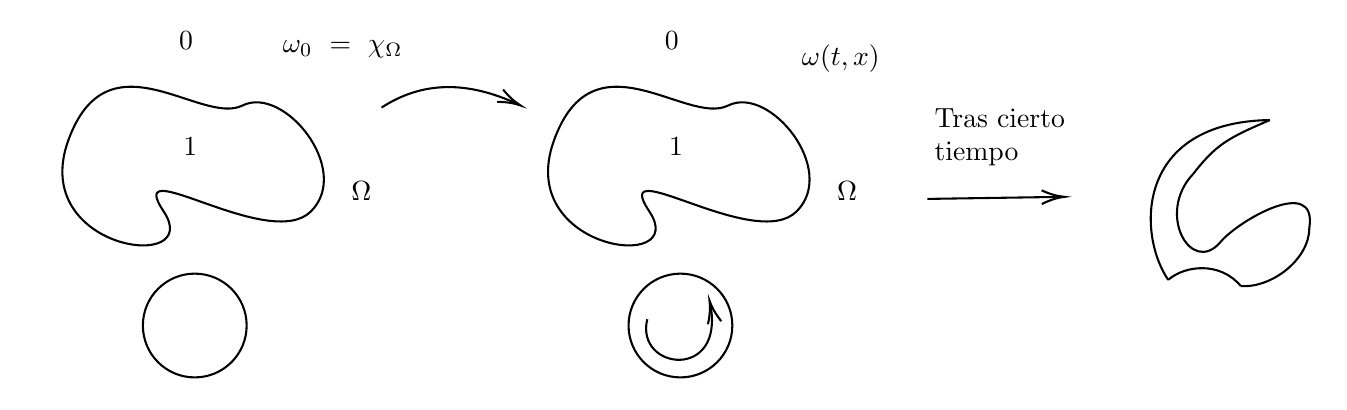
\begin{tikzpicture}[x=0.75pt,y=0.75pt,yscale=-1,xscale=1]
        %uncomment if require: \path (0,300); %set diagram left start at 0, and has height of 300

        %Shape: Polygon Curved [id:ds3053046118097098] 
        \draw   (101,86) .. controls (121,76) and (154,117) .. (134,137) .. controls (114,157) and (43,107) .. (63,137) .. controls (83,167) and (-2,156) .. (17,103) .. controls (36,50) and (81,96) .. (101,86) -- cycle ;
        %Shape: Circle [id:dp45660914167393973] 
        \draw   (53,192) .. controls (53,178.19) and (64.19,167) .. (78,167) .. controls (91.81,167) and (103,178.19) .. (103,192) .. controls (103,205.81) and (91.81,217) .. (78,217) .. controls (64.19,217) and (53,205.81) .. (53,192) -- cycle ;
        %Curve Lines [id:da39259218054114486] 
        \draw    (168,87) .. controls (187.6,74.26) and (209.12,74.01) .. (233.5,85.29) ;
        \draw [shift={(235,86)}, rotate = 205.64] [color={rgb, 255:red, 0; green, 0; blue, 0 }  ][line width=0.75]    (10.93,-3.29) .. controls (6.95,-1.4) and (3.31,-0.3) .. (0,0) .. controls (3.31,0.3) and (6.95,1.4) .. (10.93,3.29)   ;
        %Shape: Polygon Curved [id:ds4134756710331108] 
        \draw   (335,86) .. controls (355,76) and (388,117) .. (368,137) .. controls (348,157) and (277,107) .. (297,137) .. controls (317,167) and (232,156) .. (251,103) .. controls (270,50) and (315,96) .. (335,86) -- cycle ;
        %Shape: Circle [id:dp8570779698638371] 
        \draw   (287,192) .. controls (287,178.19) and (298.19,167) .. (312,167) .. controls (325.81,167) and (337,178.19) .. (337,192) .. controls (337,205.81) and (325.81,217) .. (312,217) .. controls (298.19,217) and (287,205.81) .. (287,192) -- cycle ;
        %Straight Lines [id:da4669948322720253] 
        \draw    (431,131) -- (495,130.03) ;
        \draw [shift={(497,130)}, rotate = 179.13] [color={rgb, 255:red, 0; green, 0; blue, 0 }  ][line width=0.75]    (10.93,-3.29) .. controls (6.95,-1.4) and (3.31,-0.3) .. (0,0) .. controls (3.31,0.3) and (6.95,1.4) .. (10.93,3.29)   ;
        %Curve Lines [id:da8186342329158359] 
        \draw    (547,170) .. controls (532,148) and (531,94) .. (596,93) ;
        %Curve Lines [id:da5025705863547494] 
        \draw    (582,173) .. controls (572,161) and (555,163) .. (547,170) ;
        %Curve Lines [id:da6580378891015024] 
        \draw    (615,145) .. controls (615,160) and (597,174) .. (582,173) ;
        %Curve Lines [id:da9498702609506636] 
        \draw    (615,145) .. controls (619,119) and (580,142) .. (572,152) ;
        %Curve Lines [id:da9148030838417588] 
        \draw    (559,119) .. controls (541,138) and (558,168) .. (572,152) ;
        %Curve Lines [id:da7310709300556156] 
        \draw    (559,119) .. controls (570,105) and (575,102) .. (596,93) ;
        %Curve Lines [id:da255938325673975] 
        \draw    (296,189) .. controls (290.09,213.63) and (333.66,218.85) .. (326.37,181.73) ;
        \draw [shift={(326,180)}, rotate = 77.01] [color={rgb, 255:red, 0; green, 0; blue, 0 }  ][line width=0.75]    (10.93,-3.29) .. controls (6.95,-1.4) and (3.31,-0.3) .. (0,0) .. controls (3.31,0.3) and (6.95,1.4) .. (10.93,3.29)   ;

        % Text Node
        \draw (71,100) node [anchor=north west][inner sep=0.75pt]   [align=left] {$\displaystyle 1$};
        % Text Node
        \draw (69,49) node [anchor=north west][inner sep=0.75pt]   [align=left] {$\displaystyle 0$};
        % Text Node
        \draw (119,53) node [anchor=north west][inner sep=0.75pt]   [align=left] {$\displaystyle \omega _{0} \ =\ \chi _{\Omega }$};
        % Text Node
        \draw (152,121) node [anchor=north west][inner sep=0.75pt]   [align=left] {$\displaystyle \Omega $};
        % Text Node
        \draw (305,100) node [anchor=north west][inner sep=0.75pt]   [align=left] {$\displaystyle 1$};
        % Text Node
        \draw (303,49) node [anchor=north west][inner sep=0.75pt]   [align=left] {$\displaystyle 0$};
        % Text Node
        \draw (369,55) node [anchor=north west][inner sep=0.75pt]   [align=left] {$\displaystyle \omega ( t,x)$};
        % Text Node
        \draw (386,121) node [anchor=north west][inner sep=0.75pt]   [align=left] {$\displaystyle \Omega $};
        % Text Node
        \draw (433,86) node [anchor=north west][inner sep=0.75pt]   [align=left] {Tras cierto \\tiempo};


        \end{tikzpicture}
        \caption{Ejemplo de parches de vorticidad}
        \label{fig:f31}
    \end{center}
\end{figure}

Este tipo de datos iniciales de la vorticidad\footnote{Aquellos en los que la vorticidad es función característica de un conjunto $\Omega$.} se denominan parches (o paquetes) de vorticidad\footnote{En inglés, \textit{vortex patch}.}. 
Si fuera verdad la Figura \ref{fig:f31}, lo que nos interesa es el contorno. Buscar cómo evolucionan los contornos es una rama que se denomina dinámica de contornos.
En este caso tiene soporte compacto y es integrable. \\

Para formalizar más, el espacio en que estas soluciones interesantes viven es $\omega(t=0,x) = \omega_0(x) \in L^\infty(\R^2) \cap L^1(\R^2)$. Casi no 
haría falta que fueran integrables si le añadimos soporte compacto. \\

\begin{figure}[H]
    \begin{center}
        \tikzset{every picture/.style={line width=0.75pt}} %set default line width to 0.75pt        

        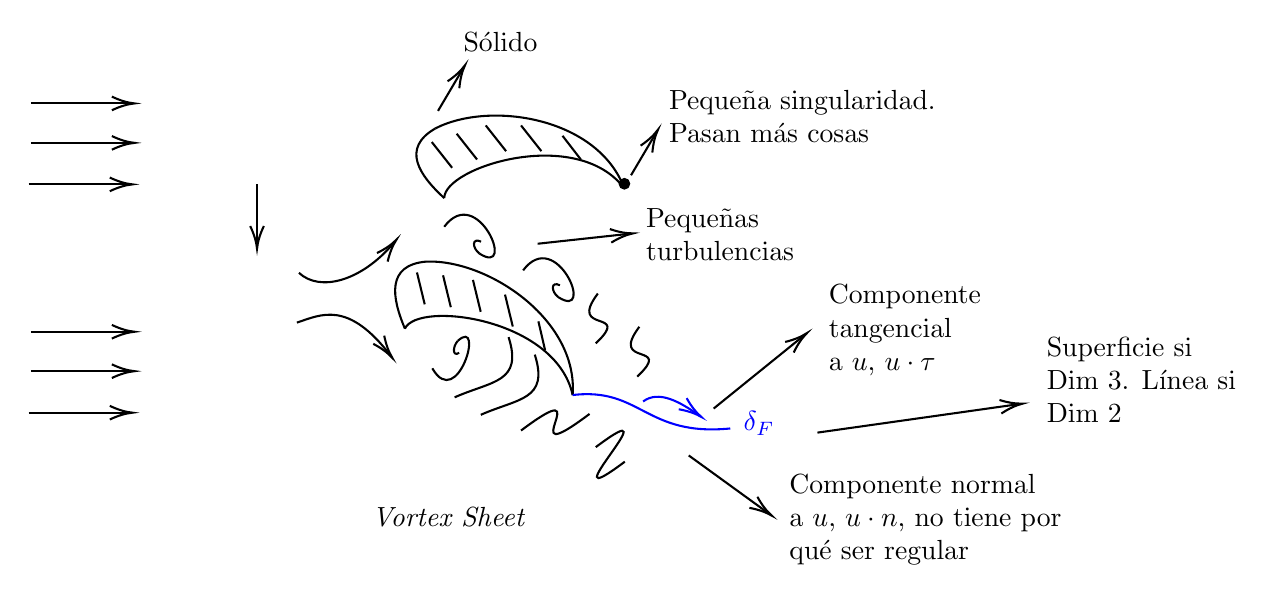
\begin{tikzpicture}[x=0.75pt,y=0.75pt,yscale=-1,xscale=1]
        %uncomment if require: \path (0,300); %set diagram left start at 0, and has height of 300

        %Straight Lines [id:da2812470710295212] 
        \draw    (31,51) -- (79,51) ;
        \draw [shift={(81,51)}, rotate = 180] [color={rgb, 255:red, 0; green, 0; blue, 0 }  ][line width=0.75]    (10.93,-3.29) .. controls (6.95,-1.4) and (3.31,-0.3) .. (0,0) .. controls (3.31,0.3) and (6.95,1.4) .. (10.93,3.29)   ;
        %Straight Lines [id:da47566060676251687] 
        \draw    (31,70) -- (79,70) ;
        \draw [shift={(81,70)}, rotate = 180] [color={rgb, 255:red, 0; green, 0; blue, 0 }  ][line width=0.75]    (10.93,-3.29) .. controls (6.95,-1.4) and (3.31,-0.3) .. (0,0) .. controls (3.31,0.3) and (6.95,1.4) .. (10.93,3.29)   ;
        %Straight Lines [id:da09091776510160365] 
        \draw    (30,90) -- (78,90) ;
        \draw [shift={(80,90)}, rotate = 180] [color={rgb, 255:red, 0; green, 0; blue, 0 }  ][line width=0.75]    (10.93,-3.29) .. controls (6.95,-1.4) and (3.31,-0.3) .. (0,0) .. controls (3.31,0.3) and (6.95,1.4) .. (10.93,3.29)   ;
        %Straight Lines [id:da15369811841719883] 
        \draw    (31,161) -- (79,161) ;
        \draw [shift={(81,161)}, rotate = 180] [color={rgb, 255:red, 0; green, 0; blue, 0 }  ][line width=0.75]    (10.93,-3.29) .. controls (6.95,-1.4) and (3.31,-0.3) .. (0,0) .. controls (3.31,0.3) and (6.95,1.4) .. (10.93,3.29)   ;
        %Straight Lines [id:da16898794784094828] 
        \draw    (31,180) -- (79,180) ;
        \draw [shift={(81,180)}, rotate = 180] [color={rgb, 255:red, 0; green, 0; blue, 0 }  ][line width=0.75]    (10.93,-3.29) .. controls (6.95,-1.4) and (3.31,-0.3) .. (0,0) .. controls (3.31,0.3) and (6.95,1.4) .. (10.93,3.29)   ;
        %Straight Lines [id:da4063777233796856] 
        \draw    (30,200) -- (78,200) ;
        \draw [shift={(80,200)}, rotate = 180] [color={rgb, 255:red, 0; green, 0; blue, 0 }  ][line width=0.75]    (10.93,-3.29) .. controls (6.95,-1.4) and (3.31,-0.3) .. (0,0) .. controls (3.31,0.3) and (6.95,1.4) .. (10.93,3.29)   ;
        %Straight Lines [id:da4020866803904283] 
        \draw    (140,90) -- (140,119) ;
        \draw [shift={(140,121)}, rotate = 270] [color={rgb, 255:red, 0; green, 0; blue, 0 }  ][line width=0.75]    (10.93,-3.29) .. controls (6.95,-1.4) and (3.31,-0.3) .. (0,0) .. controls (3.31,0.3) and (6.95,1.4) .. (10.93,3.29)   ;
        %Curve Lines [id:da15908134021767917] 
        \draw    (226,63) .. controls (252.2,49.6) and (304.2,57.6) .. (317,92) ;
        %Curve Lines [id:da21164709689584338] 
        \draw    (226,63) .. controls (209.2,72.6) and (218.2,85.6) .. (230.2,96.6) ;
        %Curve Lines [id:da8087665006399677] 
        \draw    (230.2,96.6) .. controls (230.2,81.6) and (294.2,61.6) .. (317,92) ;
        %Straight Lines [id:da9647454151853694] 
        \draw    (224.2,69.6) -- (234,82) ;
        %Straight Lines [id:da8782904375213573] 
        \draw    (236.2,65.6) -- (246,78) ;
        %Straight Lines [id:da09315412580354421] 
        \draw    (250.2,61.6) -- (260,74) ;
        %Straight Lines [id:da7099557171234606] 
        \draw    (267.2,61.6) -- (277,74) ;
        %Straight Lines [id:da32765479150297305] 
        \draw    (287.2,66.6) -- (296,78) ;
        %Straight Lines [id:da5742289166766529] 
        \draw    (227.2,54.6) -- (239.18,34.32) ;
        \draw [shift={(240.2,32.6)}, rotate = 120.58] [color={rgb, 255:red, 0; green, 0; blue, 0 }  ][line width=0.75]    (10.93,-3.29) .. controls (6.95,-1.4) and (3.31,-0.3) .. (0,0) .. controls (3.31,0.3) and (6.95,1.4) .. (10.93,3.29)   ;
        %Shape: Circle [id:dp9743827661546515] 
        \draw  [color={rgb, 255:red, 0; green, 0; blue, 0 }  ,draw opacity=1 ][fill={rgb, 255:red, 0; green, 0; blue, 0 }  ,fill opacity=1 ] (314.7,89.7) .. controls (314.7,88.43) and (315.73,87.4) .. (317,87.4) .. controls (318.27,87.4) and (319.3,88.43) .. (319.3,89.7) .. controls (319.3,90.97) and (318.27,92) .. (317,92) .. controls (315.73,92) and (314.7,90.97) .. (314.7,89.7) -- cycle ;
        %Straight Lines [id:da44093713674943735] 
        \draw    (320.2,85.6) -- (332.18,65.32) ;
        \draw [shift={(333.2,63.6)}, rotate = 120.58] [color={rgb, 255:red, 0; green, 0; blue, 0 }  ][line width=0.75]    (10.93,-3.29) .. controls (6.95,-1.4) and (3.31,-0.3) .. (0,0) .. controls (3.31,0.3) and (6.95,1.4) .. (10.93,3.29)   ;
        %Curve Lines [id:da9782551750351288] 
        \draw    (221.45,127.21) .. controls (250.85,125.95) and (294.78,154.9) .. (292.07,191.5) ;
        %Curve Lines [id:da6457406154474422] 
        \draw    (221.45,127.21) .. controls (202.17,128.93) and (204.93,144.5) .. (211.25,159.5) ;
        %Curve Lines [id:da6592127058421853] 
        \draw    (211.25,159.5) .. controls (217.51,145.86) and (284.02,154.37) .. (292.07,191.5) ;
        %Straight Lines [id:da8164395489389693] 
        \draw    (217.06,132.45) -- (220.8,147.81) ;
        %Straight Lines [id:da5997991788831862] 
        \draw    (229.63,133.82) -- (233.37,149.18) ;
        %Straight Lines [id:da21725399929697986] 
        \draw    (244.03,136.02) -- (247.76,151.38) ;
        %Straight Lines [id:da37594237267956354] 
        \draw    (259.48,143.11) -- (263.22,158.47) ;
        %Straight Lines [id:da5660065818913599] 
        \draw    (275.57,155.99) -- (278.82,170.02) ;
        %Curve Lines [id:da4348210794241574] 
        \draw    (160.2,132.6) .. controls (170.14,141.96) and (190.17,136.87) .. (205.99,118.07) ;
        \draw [shift={(207.2,116.6)}, rotate = 128.66] [color={rgb, 255:red, 0; green, 0; blue, 0 }  ][line width=0.75]    (10.93,-3.29) .. controls (6.95,-1.4) and (3.31,-0.3) .. (0,0) .. controls (3.31,0.3) and (6.95,1.4) .. (10.93,3.29)   ;
        %Curve Lines [id:da773331916689267] 
        \draw    (159.2,156.6) .. controls (171.02,152.66) and (183.81,145.81) .. (204.26,172.36) ;
        \draw [shift={(205.2,173.6)}, rotate = 233.13] [color={rgb, 255:red, 0; green, 0; blue, 0 }  ][line width=0.75]    (10.93,-3.29) .. controls (6.95,-1.4) and (3.31,-0.3) .. (0,0) .. controls (3.31,0.3) and (6.95,1.4) .. (10.93,3.29)   ;
        %Curve Lines [id:da6631647361637638] 
        \draw    (224.46,178.63) .. controls (236.65,199.82) and (249.91,153.53) .. (236.73,165.38) ;
        %Curve Lines [id:da6563990817342066] 
        \draw    (236.73,165.38) .. controls (234.1,168.32) and (234.18,173.34) .. (237.41,171.1) ;
        %Curve Lines [id:da1508397637449559] 
        \draw    (230.2,110.42) .. controls (246.34,88.9) and (265.31,134.82) .. (247.15,123.34) ;
        %Curve Lines [id:da5937672725257489] 
        \draw    (247.15,123.34) .. controls (243.52,120.47) and (243.52,115.45) .. (247.95,117.6) ;
        %Curve Lines [id:da9324690646615994] 
        \draw    (268.2,131.42) .. controls (284.34,109.9) and (303.31,155.82) .. (285.15,144.34) ;
        %Curve Lines [id:da9285295925185382] 
        \draw    (285.15,144.34) .. controls (281.52,141.47) and (281.52,136.45) .. (285.95,138.6) ;
        %Curve Lines [id:da800505442183486] 
        \draw    (303.2,166.6) .. controls (321.2,149.6) and (289.2,162.6) .. (304.2,142.6) ;
        %Curve Lines [id:da8942786587901006] 
        \draw    (323.2,182.6) .. controls (341.2,165.6) and (309.2,178.6) .. (324.2,158.6) ;
        %Straight Lines [id:da19147972215759101] 
        \draw    (275.2,118.6) -- (319.21,113.82) ;
        \draw [shift={(321.2,113.6)}, rotate = 173.8] [color={rgb, 255:red, 0; green, 0; blue, 0 }  ][line width=0.75]    (10.93,-3.29) .. controls (6.95,-1.4) and (3.31,-0.3) .. (0,0) .. controls (3.31,0.3) and (6.95,1.4) .. (10.93,3.29)   ;
        %Curve Lines [id:da7954650578120924] 
        \draw    (235.2,192.6) .. controls (253.2,184.6) and (268.2,185.6) .. (261.2,163.6) ;
        %Curve Lines [id:da9433565556338858] 
        \draw    (247.82,201.02) .. controls (265.82,193.02) and (280.82,194.02) .. (273.82,172.02) ;
        %Curve Lines [id:da48799610894319867] 
        \draw    (267.2,208.6) .. controls (307.2,178.6) and (260.2,230.6) .. (300.2,200.6) ;
        %Curve Lines [id:da2469256654584021] 
        \draw    (303.2,216.6) .. controls (343.2,186.6) and (277.2,253.6) .. (317.2,223.6) ;
        %Curve Lines [id:da31900950697469144] 
        \draw [color={rgb, 255:red, 0; green, 0; blue, 255 }  ,draw opacity=1 ]   (292.07,191.5) .. controls (325,187.6) and (327,211.6) .. (368,207.6) ;
        %Straight Lines [id:da7667827219254041] 
        \draw    (360,198) -- (403.45,162.86) ;
        \draw [shift={(405,161.6)}, rotate = 141.03] [color={rgb, 255:red, 0; green, 0; blue, 0 }  ][line width=0.75]    (10.93,-3.29) .. controls (6.95,-1.4) and (3.31,-0.3) .. (0,0) .. controls (3.31,0.3) and (6.95,1.4) .. (10.93,3.29)   ;
        %Straight Lines [id:da4619382821140623] 
        \draw    (348,220.6) -- (386.38,248.43) ;
        \draw [shift={(388,249.6)}, rotate = 215.94] [color={rgb, 255:red, 0; green, 0; blue, 0 }  ][line width=0.75]    (10.93,-3.29) .. controls (6.95,-1.4) and (3.31,-0.3) .. (0,0) .. controls (3.31,0.3) and (6.95,1.4) .. (10.93,3.29)   ;
        %Straight Lines [id:da4973385330210537] 
        \draw    (410,209.6) -- (507.02,195.88) ;
        \draw [shift={(509,195.6)}, rotate = 171.95] [color={rgb, 255:red, 0; green, 0; blue, 0 }  ][line width=0.75]    (10.93,-3.29) .. controls (6.95,-1.4) and (3.31,-0.3) .. (0,0) .. controls (3.31,0.3) and (6.95,1.4) .. (10.93,3.29)   ;
        %Curve Lines [id:da9763631526140586] 
        \draw [color={rgb, 255:red, 0; green, 0; blue, 255 }  ,draw opacity=1 ]   (326,194.6) .. controls (333.56,188.93) and (343.8,194.87) .. (352.5,200.94) ;
        \draw [shift={(354,202)}, rotate = 215.42] [color={rgb, 255:red, 0; green, 0; blue, 255 }  ,draw opacity=1 ][line width=0.75]    (10.93,-3.29) .. controls (6.95,-1.4) and (3.31,-0.3) .. (0,0) .. controls (3.31,0.3) and (6.95,1.4) .. (10.93,3.29)   ;

        % Text Node
        \draw (238,15) node [anchor=north west][inner sep=0.75pt]   [align=left] {Sólido};
        % Text Node
        \draw (337,43) node [anchor=north west][inner sep=0.75pt]   [align=left] {Pequeña singularidad.\\Pasan más cosas};
        % Text Node
        \draw (326,100) node [anchor=north west][inner sep=0.75pt]   [align=left] {Pequeñas \\turbulencias};
        % Text Node
        \draw (414,137) node [anchor=north west][inner sep=0.75pt]   [align=left] {Componente\\tangencial \\a $\displaystyle u$, $\displaystyle u\cdot \tau $};
        % Text Node
        \draw (373,198) node [anchor=north west][inner sep=0.75pt]   [align=left] {$\displaystyle \textcolor[rgb]{0,0,1}{\delta _{F}}$};
        % Text Node
        \draw (395,228) node [anchor=north west][inner sep=0.75pt]   [align=left] {Componente normal\\a $\displaystyle u$, $\displaystyle u\cdot n$, no tiene por \\qué ser regular};
        % Text Node
        \draw (519,162) node [anchor=north west][inner sep=0.75pt]   [align=left] {Superficie si \\Dim 3. Línea si \\Dim 2};
        % Text Node
        \draw (194,244) node [anchor=north west][inner sep=0.75pt]   [align=left] {\textit{Vortex Sheet}};


        \end{tikzpicture}
    \caption{Formación de una hoja de vorticidad.}
    \label{fig:f34}
    \end{center}
\end{figure}

Este tipo de fenómenos se dan cuando, por ejemplo, despega un avión. Si no se controla la hoja de vórtice\footnote{También conocida como lámina o capa de vórtices. En inglés como \textit{vortex sheet}.}, 
tiene tanta fuerza que parte el ala del avión (da igual que esté hecho de acero). El $\delta_F$ que aparece en la Figura \ref{fig:f34} es una delta de Dirac, que veremos más adelante. \\

Estos ejemplos motivan el estudio de la regularidad de la velocidad y de la vorticidad. En particular, nos interesa determinar bajo qué hipótesis sobre 
$\omega$ podemos garantizar que el campo de velocidades $(u=K*\omega)$ sea acotado y continuo. Volviendo a las ecuaciones, $u = K \ast \omega$ no depende del tiempo. 
Burgers no regulariza. Esta ecuación ($u = K \ast \omega$) es de tipo hiperbólico\footnote{Vista en Modelos Matemáticos II.}. La solución no se espera que sea continua. \\

Veamos el siguiente resultado\footnote{De momento paramos el tiempo, y luego estudiamos qué pasa con él.}:

\begin{lema}
    ·Si $\omega \in L^1(\R^2) \cap L^\infty(\R^2) \Longrightarrow u \in L^\infty$. La segunda parte nos dice que, no solo es acotada, sino que es continua.
    Además, $\norma{u}_{L^\infty} \leq \norma{\omega}_{L^1}^{1/2} \norma{\omega}_{L^\infty}^{1/2}$.
\end{lema}

\begin{proof}
    Consideramos 
    $$u(x) = \int_{\mathbb{R}^2} K(x-y)\omega(y)\,dy =
    \int\limits_{\substack{y\in\mathbb{R}^2\\|x-y|\leq d }} K(x-y)\omega(y)\,dy +
    \int\limits_{\substack{y\in\mathbb{R}^2\\|x-y| > d }} K(x-y)\omega(y)\,dy = I_1 + I_2$$
    donde $d \in \R$ es arbitrario. Como queremos ver que está acotado:
    $$|u(x)| \leq
    \int\limits_{\substack{y\in\mathbb{R}^2\\|x-y|\leq d}} |K(x-y)\omega(y)|\,dy + 
    \int\limits_{\substack{y\in\mathbb{R}^2\\|x-y| > d}} |K(x-y)\omega(y)|\,dy$$
    Tenemos que 
    $$I_1 = \int_{|x-y| \leq d} |K(x-y) \omega(y)|\,dy \leq \int_{|x-y| \leq d} \dfrac{|\omega(y)|}{2 \pi |x-y|}\,dy \stackrel{(*)}{\leq} 
    \dfrac{\norma{\omega}_{L^\infty}}{2 \pi} \int_{|x-y| \leq d} \dfrac{1}{|x-y|}\,dy$$
    donde en $(*)$ se ha usado que $\omega$ está uniformemente acotada. Para resolver la última integral que nos ha quedado pasamos a coordenadas polares.
    $$(x-y)_1 = r \cos \theta \quad (x-y)_2 = r \sen \theta$$
    y
    $$\dfrac{\norma{\omega}_{L^\infty}}{2 \pi} \int_{0}^{2 \pi} \int_{0}^{d} \dfrac{1}{r} r \,dr\,d \theta = d \norma{\omega}_{L^\infty}$$
    Veamos ahora la segunda integral:
    $$I_2 = \int_{|x-y| > d} \dfrac{|\omega(y)|}{2 \pi |x-y|}\,dy \leq \dfrac{1}{2 \pi d} \int_{|x-y| > d} |\omega(y)|\,dy \leq 
    \dfrac{\norma{\omega}_{L^1}}{2 \pi d}$$
    Juntando todo lo anterior, resulta que
    $$|u(x)| \leq d \norma{\omega}_{L^\infty} + \dfrac{\norma{\omega}_{L^1}}{2 \pi d}$$
    Y ahora buscamos el valor óptimo de $d$. Para ello, consideramos la función
    $$f(d) = d \norma{\omega}_{L^\infty} + \dfrac{\norma{\omega}_{L^1}}{2 \pi d}$$
    y estudiamos su monotonía. Como
    $$f'(d) = \norma{\omega}_{L^\infty} - \dfrac{\norma{\omega}_{L^1}}{2 \pi d^2}$$
    $$f'' > 0$$
    deducimos que 
    $$d = \sqrt{\dfrac{\norma{\omega}_{L^1}}{2 \pi \norma{\omega}_{L^\infty}}}$$
    es el valor óptimo. Por tanto,
    $$|u(x)| \leq d \norma{\omega}_{L^\infty} + \dfrac{\norma{\omega}_{L^1}}{2 \pi d} = $$
    $$\dfrac{1}{\sqrt{2 \pi}} \norma{\omega}_{L^1}^{1/2} \norma{\omega}_{L^\infty}^{1/2} + 
    \dfrac{1}{\sqrt{2 \pi}} \norma{\omega}_{L^1}^{1/2} \norma{\omega}_{L^\infty}^{1/2} = \dfrac{2}{\sqrt{2 \pi}} \norma{\omega}_{L^1}^{1/2} \norma{\omega}_{L^\infty}^{1/2} $$ 
\end{proof}

\begin{ejercicio}
    ¿Qué ocurre si $\omega \in L^p(\R^2) \cap L^q(\R^2)$?, con $1 \leq p < 2 \leq q \leq +\infty$. Demostrar que $u \in L^\infty$ ($u$ está acotada). Se hace igual, 
    pero en vez de hacer directamente acotación, hay que aplicar Hölder primero. 
\end{ejercicio}

% 26.10.2026

Tenemos también el siguiente lema:

\begin{lema}\label{lema:l1}
    Si $\omega \in L^1 \cap L^\infty$, entonces:
    $$\begin{cases}
        1)& \quad |u(t,x+y) - u(t,x)| \leq C |y| \{1 + |\ln|y||\} \\
        2)& \quad |u(t,x)| \to 0 \quad |x| \to \infty
    \end{cases}$$
    donde $C = (C(\norma{\omega}_{L^1}, \norma{\omega}_{L^\infty}))$
\end{lema}

\begin{observacion}
    La segunda propiedad se deduce de que $u = K \ast \omega$. \\
\end{observacion}

Para estudiar el lema anterior vemos primero algunas propiedades de la función $K$:

\begin{ejercicio}\label{ejercicio:ej31}
    Demostrar que 
    $$|K(a) - K(b)| \leq C \left\{ \dfrac{1}{|a|} + \dfrac{1}{|b|} \right\} \quad \forall a,b \in \R^2 \setminus \{0\}$$
    $$|K(a) - K(b)| = \dfrac{1}{2 \pi} \dfrac{|b-a|}{|a||b|}$$

    La primera propiedad es sencilla de comprobar, y la segunda se deducirá a partir de la propia definición de $K$:
    $$K(x) = \dfrac{(-x_2, x_1)}{2 \pi |x|^2}$$
\end{ejercicio}

Demostramos el Lema \ref{lema:l1}:

\begin{proof}
    Para la primera propiedad, vemos que 
    $$u(x+y) - u(x) = \int_{\R^2} (K(x+y-z) - K(x-z)) \omega(z)\,dz \Longrightarrow$$
    $$|u(x+y) - u(x)| \leq \int_{\R^2} |(K(x+y-z) - K(x-z)) \omega(z)|\,dz \leq \int_{|x-z| \leq d} + \int_{|x-z| > d} = I_1 + I_2$$
    Hacemos ya la elección $d = 2|y| << 1$. Usamos ahora la primera propiedad del Ejercicio \ref{ejercicio:ej31} para $I_1$, y nos queda
    $$I_1 \leq \dfrac{1}{2 \pi} \int_{|x-z| \leq d} \dfrac{|\omega(z)|}{|x+y-z|} + \dfrac{1}{2 \pi} \int_{|x-z| \leq d} \dfrac{|\omega(z)|}{|x-z|}$$
    Estudiamos el denominador de la primera integral que acota a $I_1$:
    $$|x+y-z| \stackrel{|x-z| \leq d}{\leq} |x-z| + |y| \leq d + \dfrac{d}{2} = \dfrac{3d}{2}$$
    y se tiene que 
    $$\dfrac{1}{2 \pi} \int_{|x-z| \leq d} \dfrac{|\omega(z)|}{|x+y-z|} + \dfrac{1}{2 \pi} \int_{|x-z| \leq d} \dfrac{|\omega(z)|}{|x-z|} \leq $$
    $$\dfrac{1}{2 \pi} \int_{|x+y-z| \leq 3d/2} \dfrac{|\omega(z)|}{|x+y-z|} + \dfrac{1}{2 \pi} \int_{|x-z| \leq d} \dfrac{|\omega(z)|}{|x-z|}$$
    Ahora aplicamos los siguientes cambios a polares:
    $$(x+y-z)_i = r \cos \theta \quad (x+y-z)_j = r \sen \theta$$
    $$(x-z)_i = r \cos \theta \quad (x-z)_j = r \sen \theta$$
    obteniendo que 
    $$\dfrac{1}{2 \pi} \int_{|x+y-z| \leq 3d/2} \dfrac{|\omega(z)|}{|x+y-z|} + \dfrac{1}{2 \pi} \int_{|x-z| \leq d} \dfrac{|\omega(z)|}{|x-z|} \leq 
    C d \norma{\omega}_{L^\infty}$$
    Repetimos este esquema con $I_2$:
    $$I_2 \leq \dfrac{1}{2 \pi} \int_{|x-z| > d} \dfrac{|y| |\omega(z)|}{|x+y-z| |x-z|} \stackrel{(*)}{=} \int_{d \leq |x-z| \leq 1} + \int_{|x-z| > 1}$$
    donde en $(*)$ se ha usado que esta división en dos partes de la integral es la que funciona.
    En este caso el denominador $|x+y-z|$ está acotado inferiormente:
    $$|x+y-z| \geq |x-z| - |y| = |x-z| - \dfrac{d}{2} \geq |x-2| - \dfrac{|x-2|}{2} = \dfrac{|x-2|}{2}$$
    de donde
    $$\int_{1 \leq |x-z| \leq d} + \int_{|x-z| > 1} \leq \dfrac{|y|}{2 \pi} \int_{d \leq |x-z| \leq 1} \dfrac{2 |\omega(z)|}{|x-z|^2} + \int_{|x-z| > 1}$$
    Integramos en cada uno de los dos trozos. En el tramo $d \leq |x-z| \leq 1$:
    $$\dfrac{|y|}{\pi} \norma{\omega}_{L^\infty} \dfrac{1}{|x-2|^2} = \dfrac{|y|}{\pi} \norma{\omega}_{L^\infty} \int_{0}^{2 \pi} \int_{d}^{1} \dfrac{1}{r^2}
    r\,dr\,d \theta = 2 |y|\norma{\omega}_{L^\infty}(-\ln \overbrace{d}^{2 |y|}) \stackrel{d < 1}{=} $$
    $$2 |y| \norma{\omega}_{L^\infty}(|\ln d|) = 2 |y| \norma{\omega}_{L^\infty} (\ln 2 + |\ln|y||)$$
    Acotando la suma anterior de integrales, nos queda:
    $$\dfrac{|y|}{2 \pi} \int_{d \leq |x-z| \leq 1} \dfrac{2 |\omega(z)|}{|x-z|^2} + \int_{|x-z| > 1} \leq \dfrac{|y|}{\pi} \norma{\omega}_{L^1}$$
    y usando entonces las cotas que tenemos para $I_1$ e $I_2$, se deduce que 
    $$|u(x+y) - u(x)| \leq \int_{\R^2} |(K(x+y-z) - K(x-z)) \omega(z)|\,dz \leq I_1 + I_2 \leq$$
    $$|y| \left\{2 C \norma{\omega}_{L^\infty} + \dfrac{\norma{\omega}_{L^1}}{\pi} + 2 \ln 2 \norma{\omega}_{L^\infty} + 
    2 \norma{\omega}_{L^\infty} |\ln|y|| \right\}$$
\end{proof}

\begin{observacion}
    Justo el hecho de que se tenga $L^1$ y $L^\infty$ nos da la unicidad. Si buscamos exámenes de años anteriores, esto se puede preguntar en el examen. 
    Siempre intenta preguntar alguna cosa de teoría y algo que haya que hacer alguna cuenta. No hay mucho que preguntar. \\
\end{observacion}

Ahora, consideramos $f \in L^1$, y, dado $\varepsilon > 0$, existe $R > 0$ con\footnote{Se lee como ``$R$ suficientemente grande''.} $R >> 1$
tal que $$\int_{|y| > R} |f(y)|\,dy < \varepsilon$$
Esto vale también para casi cualquier $L^p$, ya que vale para $1 < p < \infty$, y entonces se tiene que
$$\int_{|y| > R} |f(y)|^p\,dy < \varepsilon$$
Para una integral lo suficientemente grande, tienen tendencia a irse a $0$ para un radio lo suficientemente grande. \\

Para comprobar esto, podemos verlo como
$$\int_{|y| > R} |f(y)|\,dy = \int_{\R^2} |f(y)|\,dy - \int_{|y| < R} |f(y)|\,dy \to 0 \quad (R \to \infty)$$
Consideramos ahora $|x| > 2R$. Vemos que 
$$|u(x)| \leq \int \dfrac{|\omega(y)|}{2 \pi |x-y|}\,dy = \int_{|y| > R} + \int_{|y| < R}$$
Ahora, si $|y| < R < |x| / 2$, donde la última desigualdad se debe a que $|x| < 2R$ por hipótesis, entonces
$$|x-y| \geq |x| - |y| = |x| \left\{ 1 - \dfrac{|y|}{|x|} \right\} > \dfrac{|x|}{2}$$
y
$$\dfrac{1}{2 \pi} \int_{|y| < R} \dfrac{|\omega(y)|}{|x-y|} \leq \dfrac{1}{2 \pi} \dfrac{2}{|x|} \int_{|y| < R} |\omega(y)|$$
Nuevamente, dividimos
$$
\int_{|y|>R}
=
\int_{\substack{|y|>R\\|x-y|\leq d}}
+
\underbrace{
\int_{\substack{|y|>R\\|x-y|>d}}
\frac{|\omega(y)|}{2\pi|x-y|}
}_{(*)}
$$
De esta manera, recuperando lo anterior:
$$|u(x)| \leq \int \dfrac{|\omega(y)|}{2 \pi |x-y|}\,dy = \int_{|y| > R} + \int_{|y| < R} = \dfrac{1}{\pi} \dfrac{1}{|x|} \norma{\omega_{L^1}} + 
\overbrace{d}^{\sqrt{\varepsilon}} \norma{\omega}_{L^\infty} + \dfrac{1}{2 \pi} \dfrac{\varepsilon}{d}$$
La integral $(*)$ nos da:
$$\dfrac{1}{2 \pi} \dfrac{1}{d} \int_{|y| > R} |\omega(y)| < \varepsilon$$
y no menor que $\norma{\omega}_{L^1}$, ya que se nos iría a infinito. \\

El siguiente resultado nos resultará bastante útil en lo que sigue:
\begin{lema}
    Sean $\varphi, \psi$ dos cambios de variable en $\R^2$ con Jacobianos inversos acotados, $\omega \in L^1 \cap L^\infty$ y 
    $$\left| \int_{\R^2} (K(x - \psi(y)) - K(x - \varphi(y)))\omega(y) \right| \leq C \norma{J_\psi^{-1}}_{L^\infty}
    \norma{J_\varphi^{-1}}_{L^\infty} \norma{\psi - \varphi}_{L^\infty} \{1 + |\ln \norma{\psi - \varphi}_{L^\infty}|\}$$
    Como sugerencia estudiar el caso $\varphi = 1$.
\end{lema}

\begin{observacion}
    Este resultado es una generalización de la primera propiedad del Lema \ref{lema:l1}.
\end{observacion}

% 27.10.2026

Vamos a estudiar a continuación las siguientes ecuaciones:
\begin{equation}\label{eq:ec30}
    \begin{cases}
        \dfrac{\partial \omega}{\partial t} + (u \cdot \nabla) \omega = 0 \\
        u = K \ast \omega \\
        \omega(t=0,x) = \omega_0(x) \in L^1 \cap L^\infty
    \end{cases}
\end{equation}

Y los siguientes pasos:
\begin{enumerate}
    \item Regularización (linealización), $\varepsilon \to (u^\varepsilon, \omega^\varepsilon)$ (soluciones de un problema aproximado).
    \item Estimaciones ``a priori''.
    \item Compacidad $(u^\varepsilon, \omega^\varepsilon) \stackrel{?}{\to} (u,\omega)$.
    \item $(u, \omega)$ verifique \eqref{eq:ec30}.
\end{enumerate}

Así pues, consideramos $\varepsilon > 0$, y una función 
$$\rho \in C_0^\infty(\R^2) = \begin{cases}
    c e^{\dfrac{1}{|x|^2 - 1}} \quad& |x| \leq 1 \\
    0 \quad& |x| > 1
\end{cases}; \quad c = \left( \int_{B(0,1)} e^{\dfrac{1}{|x|^2 - 1}}  \right)^{-1} \Longrightarrow \int \rho = 1$$

Con estas funciones vamos a construir las funciones
$$C_0^\infty(B(0,\varepsilon)) \ni \rho_\varepsilon = \varepsilon^{-2} \rho \left( \dfrac{x}{\varepsilon} \right) \Longrightarrow \omega_0 \ast \rho_\varepsilon = \omega_0^\varepsilon = \omega^0$$
Gráficamente:
\begin{figure}[H]
    \begin{center}
        \tikzset{every picture/.style={line width=0.75pt}} %set default line width to 0.75pt        

        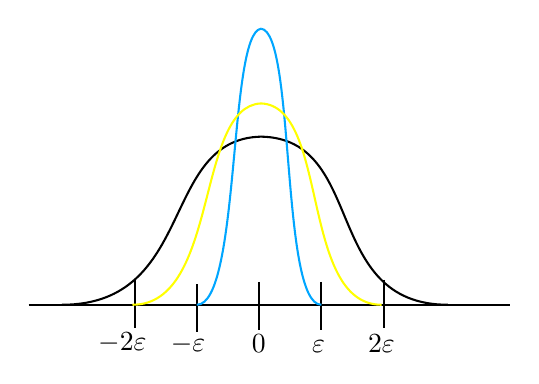
\begin{tikzpicture}[x=0.75pt,y=0.75pt,yscale=-1,xscale=1]
        %uncomment if require: \path (0,300); %set diagram left start at 0, and has height of 300

        %Straight Lines [id:da44261844071929823] 
        \draw    (179,160) -- (411,160) ;
        %Straight Lines [id:da6567160598379451] 
        \draw    (290,149) -- (290,172) ;
        %Straight Lines [id:da7983049400227261] 
        \draw    (320,149) -- (320,172) ;
        %Straight Lines [id:da22603462141458197] 
        \draw    (260,150) -- (260,173) ;
        %Straight Lines [id:da19826657884532428] 
        \draw    (230,148) -- (230,171) ;
        %Straight Lines [id:da21094039468564174] 
        \draw    (350,148) -- (350,171) ;
        %Curve Lines [id:da1863316553924157] 
        \draw    (195,160) .. controls (260,160) and (242,80) .. (291,79) ;
        %Curve Lines [id:da3633895598898311] 
        \draw    (381,160) .. controls (320,160) and (342,80) .. (291,79) ;
        %Curve Lines [id:da9557797216212501] 
        \draw [color={rgb, 255:red, 0; green, 166; blue, 255 }  ,draw opacity=1 ]   (260,160) .. controls (280.97,160) and (275.16,28.64) .. (290.97,27) ;
        %Curve Lines [id:da5860357687341343] 
        \draw [color={rgb, 255:red, 0; green, 166; blue, 255 }  ,draw opacity=1 ]   (320,160) .. controls (300.32,160) and (307.42,28.64) .. (290.97,27) ;
        %Curve Lines [id:da4852955872046737] 
        \draw [color={rgb, 255:red, 255; green, 255; blue, 0 }  ,draw opacity=1 ]   (229,160) .. controls (270.94,160) and (259.32,64.2) .. (290.94,63) ;
        %Curve Lines [id:da8261174027182207] 
        \draw [color={rgb, 255:red, 255; green, 255; blue, 0 }  ,draw opacity=1 ]   (349,160) .. controls (309.65,160) and (323.84,64.2) .. (290.94,63) ;

        % Text Node
        \draw (285,173) node [anchor=north west][inner sep=0.75pt]   [align=left] {$\displaystyle 0$};
        % Text Node
        \draw (314,176) node [anchor=north west][inner sep=0.75pt]   [align=left] {$\displaystyle \varepsilon $};
        % Text Node
        \draw (246,173) node [anchor=north west][inner sep=0.75pt]   [align=left] {$\displaystyle -\varepsilon $};
        % Text Node
        \draw (211,172) node [anchor=north west][inner sep=0.75pt]   [align=left] {$\displaystyle -2\varepsilon $};
        % Text Node
        \draw (341,173) node [anchor=north west][inner sep=0.75pt]   [align=left] {$\displaystyle 2\varepsilon $};


        \end{tikzpicture}
    \end{center}
\end{figure}
Respecto a la definición de $\rho_\varepsilon$, tenemos que 
$$\varphi \in C_0^0 \Longrightarrow \prodescalar{\rho_\varepsilon}{\varphi} = \int \rho_\varepsilon \varphi \Longrightarrow \lim\limits_{\varepsilon \to 0} \int_{\R^2} \rho_\varepsilon(x) \varphi(x)\,dx = \varphi(0) = \prodescalar{\delta_{x = 0}}{\varphi}$$
donde $\delta$ es la delta de Dirac\footnote{La delta de Dirac es una distribución caracterizada por $\langle \delta_0,\varphi\rangle=\varphi(0)$ para toda función test $\varphi$.}.
Sabemos que 
$$\norma{\omega_0^\varepsilon - \omega_0}_{L^p} \to 0 \quad 1 \leq p < +\infty$$
Si consideramos el intervalo $[0, \varepsilon]$\footnote{Tiempo muy pequeño.}, tenemos el siguiente problema:
\begin{equation}
    (P_1) \begin{cases}
        \dfrac{\partial \omega^1}{\partial t} + (u^0 \cdot \nabla) \omega^1 = 0 \\
        u^0 = K \ast \omega^0 \text{ (dado)}\\
        \omega^1(t=0,x) = \omega^0(x)
    \end{cases}
\end{equation}

Lo importante es que $u^0$ no depende del tiempo, y las funciones con superíndice $0$ están dadas. La velocidad es la convolución con la vorticidad.
Lo único que hemos hecho es retrasar la velocidad un poco en el tiempo. Si esto funciona, la idea es continuar en los siguientes pasos. Ahora consideramos
el intervalo $[\varepsilon, 2 \varepsilon]$, y tenemos en este caso el problema:
\begin{equation}
    (P_2) \begin{cases}
        \dfrac{\partial \omega^2}{\partial t} + (u^1 \cdot \nabla) \omega^2 = 0 \\
        u^1 = K \ast \omega^1(\varepsilon, \cdot)\\
        \omega^2(\varepsilon,x) = \omega^1(\varepsilon, x)
    \end{cases}
\end{equation}

Repitiendo hasta $n$ veces, y situándonos entonces en el intervalo $[(n-1)\varepsilon, n \varepsilon]$ llegamos al problema:
\begin{equation}
    (P_n) \begin{cases}
        \dfrac{\partial \omega^n}{\partial t} + (u^{n-1} \cdot \nabla) \omega^n = 0 \\
        u^{n-1} = K \ast \omega^{n-1}((n-1)\varepsilon, \cdot)\\
        \omega^n((n-1)\varepsilon,x) = \omega^{n-1}((n-1)\varepsilon, x)
    \end{cases}
\end{equation}

De aquí llegamos a las siguientes ecuaciones:
\begin{equation}\label{eq:ec31}
    \begin{cases}
        \dfrac{d X^0(t)}{dt} = u^0(X^0(t)) \\
        X^0(0) = x
    \end{cases} \quad t \in [0,\varepsilon]
\end{equation}

Ahora, dado que $\omega_0 \in L^1 \cap L^\infty$, podemos ver si en norma está acotado:
$$\norma{\omega^0}_{L^1} = \norma{\omega_0 \ast \rho_\varepsilon}_{L^1} \leq \norma{\omega_0}_{L^1} \overbrace{\norma{\rho_\varepsilon}_{L^1}}^{1}$$
$$\norma{\omega^0}_{L^\infty} = \norma{\omega_0 \ast \rho_\varepsilon}_{L^\infty} \leq \norma{\omega_0}_{L^\infty} 
\overbrace{\norma{\rho_\varepsilon}_{L^1}}^{1}$$
Por lo tanto, $\omega^0 \in L^1 \cap L^\infty$ independientemente de $\varepsilon$. \\

Esto lo resumimos en el siguiente lema:
\begin{lema}
    Sea $\omega^0 \in L^1 \cap L^\infty$. Entonces se tiene que 
    \begin{equation*}
        \begin{cases}
            u^0 \in L^\infty \\
            |u^0(x+y) - u^0(x)| \leq C |y| \{1 + |\ln|y||\} \\
            |u^0(x)| \to 0 \quad |x| \to \infty \\
            \di(u^0) = 0
        \end{cases} \quad C = C(\norma{\omega^0}_{L^1}, \norma{\omega^0}_{L^\infty})
    \end{equation*}
    Y además, existe una única solución $X^0$ de \eqref{eq:ec31}.
\end{lema}

\begin{observacion}
    $\di(u^0) = 0$, porque $K$ es un rotacional, y vimos en el Ejercicio \ref{ejercicio:ej12} apartado (i) que la divergencia del rotacional es $0$.
\end{observacion}

\begin{proof}
    Vemos que 
    $$\dfrac{d}{dt} \omega^1(t, X^0(t)) = \left( \dfrac{\partial \omega^1}{\partial t} + \left( \dfrac{\partial X^0}{\partial t} \cdot \nabla \right)
    \omega^1 \right)(t, X^0(t)) = 0$$
    Y ya tenemos la solución de este problema, pues 
    $$\omega^1(t, X^0(t)) = \omega^1(0, X^0(0)) = \omega^0(x)$$
\end{proof}

\begin{observacion}
    Para cada $\varepsilon$ fijo, $u^0$ ya es infinitamente derivable en \eqref{eq:ec30}. Además, $X$ es un difeomorfismo, y podemos hacer un 
    cambio de variable si fuera necesario. Dicho cambio sería el siguiente:
    $$y = X^0(t; 0, x) = X^0(t) \Longrightarrow x = X^0(0; t,y)$$
    Así, aplicando el cambio:
    $$\omega^1(t,y) = \omega^0(X^0(0;t,y))$$
\end{observacion}

Lo anterior vale para un tiempo muy pequeño $[0, \varepsilon]$. Ahora nos preguntamos por el valor de la norma de $\omega^1$, 
con objeto de seguir estudiando propiedades:
$$\norma{\omega^1(t, \cdot)}_{L^1} = \norma{\omega^0(X^0(0; t, y))}_{L^1} = \int_{\R^2} |\omega^0(X^0(0;t,y))|\,dy = $$
$$\int_{\R^2} |\omega^0(z)| \overbrace{J_{x^0}}^{1}\,dz = \norma{\omega^0}_{L^1}$$
Lo anterior vale para la norma en $L^1$, pero en $L^\infty$ es análogo, pues:
$$\norma{\omega^1(t, \cdot)}_{L^\infty} = \sup_{y \in \R^2} |\omega^0(X^0(0;t,y))| = \sup_{z \in \R^2} |\omega^0(z)| = \norma{\omega^0}_{L^\infty}$$
es decir, las normas se preservan. \\

Este procedimiento además se puede implementar con numérico. En realidad lo que hay que resolver es \eqref{eq:ec30}. Lo demás viene como 
consecuencia de esta resolución. Podemos en este punto enunciar el siguiente resultado:

\begin{notacion}
    Dado el par $(u^\varepsilon, \omega^\varepsilon)(t,x)$, si $t \in [(n-1)\varepsilon, n \varepsilon]$, con $n = 1, \ldots, [T/\varepsilon] = N$,
    donde $[\cdot]$ denota a la parte entera, entonces 
    $$(u^\varepsilon, \omega^\varepsilon) \stackrel{not}{\equiv} (u^{n-1}, \omega^n)$$
    Asimismo, denotamos 
    \begin{equation*}
        \begin{cases}
            \dfrac{\partial \omega^\varepsilon}{\partial t} + (u^\varepsilon \cdot \nabla) \omega^\varepsilon = 0 \\ 
            u^\varepsilon = K \ast \omega^\varepsilon
        \end{cases}
        \iff 
        \begin{cases}
            \dfrac{\partial \omega^n}{\partial t} + (u^{n-1} \cdot \nabla) \omega^n = 0 \\ 
            u^{n-1} = K \ast \omega^{n}(n\varepsilon)
        \end{cases}
    \end{equation*}
\end{notacion}

\begin{observacion}
    No ponemos la condición inicial porque se va obteniendo iterativamente, pero la primera condición inicial es $\omega^\varepsilon(t=0,x) =
    \omega^0(x)$, y entonces tenemos:
    \begin{equation*}
        \begin{cases}
            \dfrac{\partial \omega^\varepsilon}{\partial t} + (u^\varepsilon \cdot \nabla) \omega^\varepsilon = 0 \\ 
            u^\varepsilon = K \ast \omega^\varepsilon \\
            \omega^\varepsilon(t=0,x) = \omega^0(x)
        \end{cases}
    \end{equation*}
    y los pares $\{(u^\varepsilon, \omega^\varepsilon)\}_{\varepsilon > 0}$.
\end{observacion}

Tenemos el siguiente lema:

\begin{lema}\label{lema:l31}
    Sea $\omega_0 \in L^1 \cap L^\infty$. Se verifica que existe $C (\in \R)$ independiente de $\varepsilon$ tal que 
    \begin{enumerate}
        \item $\norma{u^\varepsilon}_{L^\infty} \leq C$
        \item $$\norma{\omega^\varepsilon(t, \cdot)}_{L^1} = \norma{\omega^0}_{L^1} \quad (\norma{\omega^{n+1}(t, \cdot)}_{L^1} = \norma{\omega^n}_{L^1})$$
        $$\norma{\omega^\varepsilon(t, \cdot)}_{L^\infty} = \norma{\omega^0}_{L^\infty} \quad (\norma{\omega^{n+1}(t, \cdot)}_{L^\infty} = \norma{\omega^n}_{L^\infty})$$
        \item $|u^\varepsilon(x) - u^\varepsilon(y)| \leq C|x-y|\{1 + |\ln|x-y||\}$
        \item $|u^p(x) - u^q(x)| \leq C |p \varepsilon - q \varepsilon| \{1 + |\ln|p \varepsilon - q \varepsilon||\}$
    \end{enumerate}
\end{lema}

\begin{observacion}
    En el punto 4., al poner $p$ como superíndice, estamos definiendo $u^p$ en el intervalo $[(p-2)\varepsilon, (p-1)\varepsilon]$, y análogo con $q$.
\end{observacion}

La Figura \ref{fig:f32} nos muestra que en cada intervalo $\left[(n-1)\varepsilon, n\varepsilon \right]$, el campo de velocidades aproximado $u^\varepsilon$ depende de la variable espacial, pero permanece constante respecto del tiempo.

\begin{figure}[H]
    \begin{center}
        \tikzset{every picture/.style={line width=0.75pt}} %set default line width to 0.75pt        

        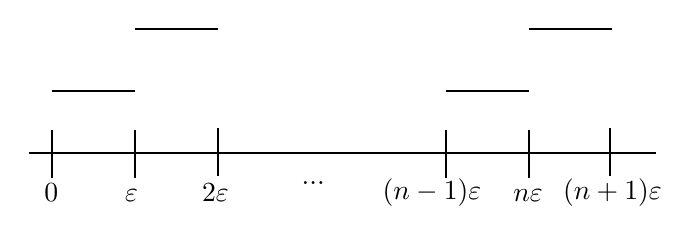
\begin{tikzpicture}[x=0.75pt,y=0.75pt,yscale=-1,xscale=1]
        %uncomment if require: \path (0,300); %set diagram left start at 0, and has height of 300

        %Straight Lines [id:da44261844071929823] 
        \draw    (150,160) -- (452,160) ;
        %Straight Lines [id:da6567160598379451] 
        \draw    (161,149) -- (161,172) ;
        %Straight Lines [id:da7983049400227261] 
        \draw    (201,149) -- (201,172) ;
        %Straight Lines [id:da21094039468564174] 
        \draw    (241,148) -- (241,171) ;
        %Straight Lines [id:da6065593239600682] 
        \draw    (351,149) -- (351,172) ;
        %Straight Lines [id:da8139488212809114] 
        \draw    (391,149) -- (391,172) ;
        %Straight Lines [id:da33702440515964105] 
        \draw    (430,148) -- (430,171) ;
        %Straight Lines [id:da8105430731321772] 
        \draw    (161,130) -- (201,130) ;
        %Straight Lines [id:da1927654285774716] 
        \draw    (201,100) -- (241,100) ;
        %Straight Lines [id:da6364192335175295] 
        \draw    (351,130) -- (391,130) ;
        %Straight Lines [id:da37849782165622403] 
        \draw    (391,100) -- (431,100) ;

        % Text Node
        \draw (156,173) node [anchor=north west][inner sep=0.75pt]   [align=left] {$\displaystyle 0$};
        % Text Node
        \draw (195,176) node [anchor=north west][inner sep=0.75pt]   [align=left] {$\displaystyle \varepsilon $};
        % Text Node
        \draw (232,173) node [anchor=north west][inner sep=0.75pt]   [align=left] {$\displaystyle 2\varepsilon $};
        % Text Node
        \draw (319,171) node [anchor=north west][inner sep=0.75pt]   [align=left] {$\displaystyle ( n-1) \varepsilon $};
        % Text Node
        \draw (382,176) node [anchor=north west][inner sep=0.75pt]   [align=left] {$\displaystyle n\varepsilon $};
        % Text Node
        \draw (406,171) node [anchor=north west][inner sep=0.75pt]   [align=left] {$\displaystyle ( n+1) \varepsilon $};
        % Text Node
        \draw (280,172) node [anchor=north west][inner sep=0.75pt]   [align=left] {...};

        \end{tikzpicture}
        \caption{Evolución temporal de $u^\varepsilon$.}
        \label{fig:f32}
    \end{center}
\end{figure}

Usamos 4 del lema anterior con $q = n$, y $p = n+1$. Tenemos que 
$$u^{n+1}(x) - u^n(x) = \int_{\R^2} K(x-y) \left( 
\underbrace{\omega^{n+1} ((n+1)\varepsilon, y)}_{\omega^{n+1}(n \varepsilon, X^n(n \varepsilon, (n+1)\varepsilon, y))} - \omega^{n} (n\varepsilon, y) \right)\,dy$$
y a su vez $\omega^{n+1}(n \varepsilon, X^n(n \varepsilon, (n+1)\varepsilon, y)) = \omega^{n}(n \varepsilon, X^n(n \varepsilon, (n+1)\varepsilon, y))$. Y ahora nos preguntamos 
por qué no podemos hacer la diferencia entre $\omega^{n}(n \varepsilon, X^n(n \varepsilon, (n+1)\varepsilon, y))$ y $\omega^n(n\varepsilon, y)$.
Se debe a que estamos en un problema hiperbólico y solo se transportan las normas, pero no podemos controlar la diferencia. Hacemos el siguiente 
cambio de variable: $z = X^n(n \varepsilon, (n+1)\varepsilon, y)$. Nos queda 
$$\int_{\R^2} K(x - X^n(n \varepsilon, (n+1)\varepsilon, z)) \omega^n(n \varepsilon, z) \overbrace{J^{-1}_{X^n}}^{1}\,dz - 
\int_{\R^2} K(x - \overbrace{y}^{z}) \omega^n(n \varepsilon, \overbrace{y}^{z})\,d\overbrace{y}^{z} = $$
$$\int_{\R^2} [K(x - \overbrace{X^n(n \varepsilon, (n+1)\varepsilon, z)}^{\psi = I_d}) - K(x-z)] \omega^n(n \varepsilon, z) \,dz$$
y aplicando el resultado anterior y conviertiendo las igualdades en desigualdades (por monotonía de la integral):
$$|u^{n+1}(x) - u^n(x)| \leq \int_{\R^2} 
\left| [K(x - \overbrace{X^n(n \varepsilon, (n+1)\varepsilon, z)}^{\psi = I_d}) - K(x-z)] \omega^n(n \varepsilon, z) \right|\,dz \leq$$
$$C \max_{z} |X^n((n+1)\varepsilon, n \varepsilon, z) - z| \{1 + |\ln \max_z |X^n((n+1)\varepsilon, n \varepsilon, z) - z||\}$$
Para ver cuánto vale ese máximo, reescribimos el argumento:
$$X^n((n+1)\varepsilon, n \varepsilon, z) - \overbrace{z}^{X^n(n \varepsilon, n \varepsilon, z)} \stackrel{TFC}{=} 
\int_{n \varepsilon}^{(n+1)\varepsilon} \dfrac{\partial}{\partial t} X^n(s, n \varepsilon, z)\,ds = 
\int_{n \varepsilon}^{(n+1)\varepsilon} u^n(s, X(s, n \varepsilon, z))\,ds$$
de donde
$$|X^n((n+1)\varepsilon, n \varepsilon, z) - z| \stackrel{(*)}{\leq} \int_{n \varepsilon}^{(n+1)\varepsilon} C \,ds = C \varepsilon$$
donde en $(*)$ se ha usado la propiedad $1$ del lema anterior. \\

\begin{observacion}
    Esta demostración es típica de examen.
\end{observacion}

% Demostración típica de examen esta dice. Entender lo que estamos haciendo.

Como $$\norma{\omega^0}_{L^1} = \norma{\omega_0 \ast \rho_\varepsilon}_{L^1} \leq \norma{\omega}_{L^1} \overbrace{\norma{\rho_\varepsilon}_{L^1}}^{1}$$
Y se puede cambiar $L^1$ por $L^\infty$. \\

Vamos a intentar aplicar ahora el Teorema de Ascoli-Arzelà, que recordemos que nos decía, dada una sucesión de funciones continuas
$\{f_\varepsilon\}_{\varepsilon \geq 0}$, que está uniformemente acotada y es equicontinua, entonces existe una parcial (que denotamos 
de la misma forma) tal que $\{f_\varepsilon\} \stackrel{c.u.}{\to} f$ sobre compactos. \\

Para nuestra sucesión, debe ser continua \textbf{en las dos variables}. En espacio lo es, pero no en tiempo, por lo que no podríamos 
aplicar el Teorema anterior directamente. Sí que será equicontinua, pero en tiempo no. Para poder aplicarlo, vamos a cambiar la regularización 
que hemos hecho. ¿Cómo podemos cambiar la $u^\varepsilon$ que tenemos hasta ahora para que sea continua? Lo más sencillo sería haciendo una 
poligonal entre puntos medios de cada intervalo $[n \varepsilon, (n+1)\varepsilon]$. Gráficamente hacemos lo que nos indica la Figura \ref{fig:f33}:

\begin{figure}[H]
    \begin{center}
        \tikzset{every picture/.style={line width=0.75pt}} %set default line width to 0.75pt        

        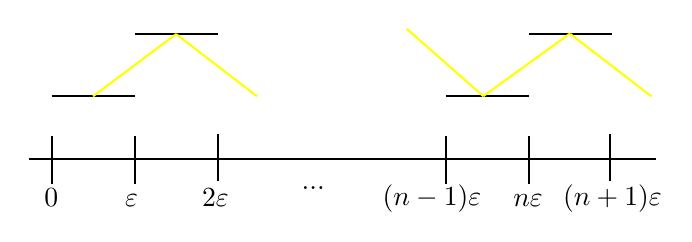
\begin{tikzpicture}[x=0.75pt,y=0.75pt,yscale=-1,xscale=1]
            %uncomment if require: \path (0,300); %set diagram left start at 0, and has height of 300

            %Straight Lines [id:da44261844071929823] 
            \draw    (150,160) -- (452,160) ;
            %Straight Lines [id:da6567160598379451] 
            \draw    (161,149) -- (161,172) ;
            %Straight Lines [id:da7983049400227261] 
            \draw    (201,149) -- (201,172) ;
            %Straight Lines [id:da21094039468564174] 
            \draw    (241,148) -- (241,171) ;
            %Straight Lines [id:da6065593239600682] 
            \draw    (351,149) -- (351,172) ;
            %Straight Lines [id:da8139488212809114] 
            \draw    (391,149) -- (391,172) ;
            %Straight Lines [id:da33702440515964105] 
            \draw    (430,148) -- (430,171) ;
            %Straight Lines [id:da8105430731321772] 
            \draw    (161,130) -- (201,130) ;
            %Straight Lines [id:da1927654285774716] 
            \draw    (201,100) -- (241,100) ;
            %Straight Lines [id:da6364192335175295] 
            \draw    (351,130) -- (391,130) ;
            %Straight Lines [id:da37849782165622403] 
            \draw    (391,100) -- (431,100) ;
            %Straight Lines [id:da9413423297139589] 
            \draw [color={rgb, 255:red, 255; green, 255; blue, 0 }  ,draw opacity=1 ]   (181,130) -- (221,100) ;
            %Straight Lines [id:da8346763639936287] 
            \draw [color={rgb, 255:red, 255; green, 255; blue, 0 }  ,draw opacity=1 ]   (221,100) -- (260,130) ;
            %Straight Lines [id:da8941574642140017] 
            \draw [color={rgb, 255:red, 255; green, 255; blue, 0 }  ,draw opacity=1 ]   (410.91,99.65) -- (369.01,129.93) ;
            %Straight Lines [id:da354821223796264] 
            \draw [color={rgb, 255:red, 255; green, 255; blue, 0 }  ,draw opacity=1 ]   (369.01,129.93) -- (332.08,97.42) ;
            %Straight Lines [id:da41995666922666564] 
            \draw [color={rgb, 255:red, 255; green, 255; blue, 0 }  ,draw opacity=1 ]   (411,100) -- (450,130) ;

            % Text Node
            \draw (156,173) node [anchor=north west][inner sep=0.75pt]   [align=left] {$\displaystyle 0$};
            % Text Node
            \draw (195,176) node [anchor=north west][inner sep=0.75pt]   [align=left] {$\displaystyle \varepsilon $};
            % Text Node
            \draw (232,173) node [anchor=north west][inner sep=0.75pt]   [align=left] {$\displaystyle 2\varepsilon $};
            % Text Node
            \draw (319,171) node [anchor=north west][inner sep=0.75pt]   [align=left] {$\displaystyle ( n-1) \varepsilon $};
            % Text Node
            \draw (382,176) node [anchor=north west][inner sep=0.75pt]   [align=left] {$\displaystyle n\varepsilon $};
            % Text Node
            \draw (406,171) node [anchor=north west][inner sep=0.75pt]   [align=left] {$\displaystyle ( n+1) \varepsilon $};
            % Text Node
            \draw (280,172) node [anchor=north west][inner sep=0.75pt]   [align=left] {...};
        \end{tikzpicture}
        \caption{Poligonales para tratar de obtener la continuidad de $u^\varepsilon$.}
        \label{fig:f33}
    \end{center}
\end{figure}

Así, la nueva definición de $u^\varepsilon$ será la siguiente:
\begin{equation*}
    \bar{u}^\varepsilon(t,x) = \begin{cases}
        u^0(x) \quad& t \in \left[0, \dfrac{\varepsilon}{2} \right]\\\\
        u^0(x) + \dfrac{t - \varepsilon/2}{\varepsilon} \left(u^1(x) - u^0(x) \right) \quad& t \in \left[\dfrac{\varepsilon}{2}, \dfrac{3\varepsilon}{2} \right]  \\\\
        \vdots \\
        u^j(x) + \dfrac{t - (j + \frac{1}{2})\varepsilon}{\varepsilon} \left(u^{j+1}(x) - u^{j}(x) \right) \quad& t \in \left[\left( j + \dfrac{1}{2} \right)\varepsilon, \left( j + \dfrac{3}{2} \right)\varepsilon \right]
    \end{cases}
\end{equation*}

\begin{lema}
    Sea $\omega_0 \in L^1 \cap L^\infty$, entonces 
    $$\norma{u^\varepsilon(t,x) - \bar{u}^{\varepsilon}(t,x)}_{L^\infty} \leq C \varepsilon |\ln \varepsilon| \stackrel{\varepsilon \to 0}{\to} 0$$
\end{lema}

Hemos cambiado $(u^\varepsilon, \omega^\varepsilon) \to (\bar{u}^\varepsilon, \omega^\varepsilon)$, y a esta sí se le puede aplicar Ascoli-Arzelà.

\begin{ejercicio}
    Comprobar el lema anterior.
\end{ejercicio}

\begin{ejercicio}
    Comprobar la equicontinuidad de $\bar{u}^\varepsilon$.
    $$|\bar{u}^\varepsilon(t,x) - \bar{u}^\varepsilon(s,x)| \leq C |t-s| \{1 + |\ln|t-s||\}$$
\end{ejercicio}

% 3.11.2026

% TODO: Revisar en lo de hoy cuándo la C es mayúscula y cuándo c es minúscula.

% TODO: Meter Dibujo 1 EDMB 3.11.2026

Teníamos que, para $t \in \left[ \left(j + \dfrac{1}{2}\right)\varepsilon, \left(j + \dfrac{3}{2}\right)\varepsilon \right]$, entonces:
% TODO: Añadir módulos para la acotación
$$u^j \left(j + \dfrac{3}{2} \right) - u^{j+1} \left(j + \dfrac{1}{2} \right) + t \left( \dfrac{u^{j+1} - u^j}{\varepsilon} \right) - $$
$$
\begin{cases}
    u^j \quad &t \in \left[ j \varepsilon, \left(j + \dfrac{1}{2} \right)\varepsilon \right[ \\\\
    u^{j+1} \quad &t \in \left] \left(j + \dfrac{1}{2} \right)\varepsilon, \left(j + 1 \right)\varepsilon \right]
\end{cases} = 
\begin{cases}
    (u^{j} - u^{j+1}) \left( j + \dfrac{1}{2} \right) + t \dfrac{u^{j+1} - u^j}{\varepsilon} \\\\
    (u^{j} - u^{j+1}) \left( j + \dfrac{3}{2} \right) + t \dfrac{u^{j+1} - u^j}{\varepsilon}
\end{cases} = $$
$$
\begin{cases}
    (u^{j+1} - u^{j}) \left( \dfrac{t}{\varepsilon} - \left( j + \dfrac{1}{2} \right) \right) \\\\
    (u^{j+1} - u^{j}) \left( \dfrac{t}{\varepsilon} - \left( j + \dfrac{3}{2} \right) \right)
\end{cases} \leq 
\begin{cases}
    \overbrace{C}^{2(j + 1/2)} |u^{j+1} - u^j| \\
    \overbrace{C}^{j + 2} |u^{j+1} - u^j|
\end{cases} < C \varepsilon(1 + |\ln \varepsilon|)$$
y podemos aplicar 4 del Lema \ref{lema:l31}. Podemos demostrar ahora que 
$$|\bar{u}^\varepsilon(t,x) - \bar{u}^\varepsilon(s,x)| \leq C |t-s| \{1 + |\ln|t-s||\}$$
Esta diferencia nos interesa calcularla cuando $t$ y $s$ estén cerca. Si están lejos nos va a dar igual. Esto se debe a que queremos 
un módulo de continuidad de $\bar{u}^\varepsilon$. Supongamos entonces que 
$$t,s \in \left[ \left(j + \dfrac{1}{2}\right)\varepsilon, \left(j + \dfrac{3}{2}\right)\varepsilon \right]$$
Entonces:
$$\left|u^j \left(j + \dfrac{3}{2} \right) - u^{j+1} \left(j + \dfrac{1}{2} \right) + t \left( \dfrac{u^{j+1} - u^j}{\varepsilon} \right) - 
\left[ u^{j} \left( j + \dfrac{3}{2} \right) - u^{j+1} \left( j + \dfrac{1}{2} \right) + s \left( \dfrac{u^{j+1} - u^j}{\varepsilon} \right) \right] \right| = $$
$$\left| (t-s) \left( \dfrac{u^{j+1} - u^j}{\varepsilon} \right) \right| \leq C |t-s| \dfrac{\varepsilon \{1 + |\ln \varepsilon|\}}{\varepsilon} \leq
C |t-s| \{1 + |\ln|t-s||\}$$

% TODO: Completar el segundo caso en que están en distintos tramos (2) del dibujo.

% TODO: Meter Dibujo 1 EDMB 3.11.2026

En un resumen de lo que conocemos hasta ahora, tenemos la siguiente proposición:

\begin{prop}
    Sea $\omega_0 \in L^1 \cap L^\infty$. Podemos construir, para cada $\varepsilon > 0$, el par $(\bar{u}^\varepsilon, \omega^\varepsilon)$ tal que:
    \begin{enumerate}
        \item $\norma{\omega^\varepsilon(t, \cdot)}_{L^1} = \norma{\omega^0}_{L^1} \leq \norma{\omega_0}_{L^1}$, y 
        $$\norma{\omega^\varepsilon(t, \cdot)}_{L^\infty} = \norma{\omega^0}_{L^\infty} \leq \norma{\omega_0}_{L^\infty}$$
        \item $\norma{\bar{u}^\varepsilon}_{L^\infty} \leq C$
        \item $|\bar{u}^\varepsilon(t,x) - \bar{u}^\varepsilon(t,y)| \leq c|x-y| \{1 + |\ln|x-y||\}$.
        \item $|\bar{u}^\varepsilon(t,x) - \bar{u}^\varepsilon(s,x)| \leq C|x-y| \{1 + |\ln|t-s||\}$.
    \end{enumerate} 
    donde $C = C(\norma{\omega_0}_{L^1}, \norma{\omega_0}_{L^\infty})$ es independiente de $\varepsilon$.
\end{prop}

\begin{observacion}
    Estas cuatro propiedades son estimaciones \underline{a priori}, debido a que las soluciones son aproximadas.
\end{observacion}

Estudiamos ahora la compacidad, con objeto a su vez de ver cuánto vale el límite de dicha sucesión. Para ello, vamos a aplicarle 
el Teorema de Ascoli-Arzelà a $\bar{u}^\varepsilon$. Recordemos que la sucesión $\{f_\varepsilon\}$ debe ser uniformemente acotada y 
equicontinua\footnote{Una sucesión de funciones $\{f_\varepsilon\}$, pongamos, $f_\varepsilon : I \to \R^N$, con $I$ un intervalo, es equicontinua si, para todo $\alpha > 0$, 
existe $\delta > 0$, con $|x-y| < \delta$ y $$|f_\varepsilon(x) - f_\varepsilon(y)| \leq \alpha \quad \forall x,y \in I$$}.
Entonces dicho teorema nos dice que existe una parcial $\{f_{\varepsilon'}\}$ tal que $f_{\varepsilon'} \stackrel{c.u.}{to} f$ en compactos. \\

Así, veamos primero que $\bar{u}^\varepsilon$ está uniformemente acotada. Dado $\alpha > 0$, nos preguntamos si existe $\delta > 0$ tal que $|x-y| < \delta$ y
$$|\bar{u}^\varepsilon(t,x) - \bar{u}^\varepsilon(t,y)| \leq C |x-y|\{1 + |\ln|x-y||\} < \alpha$$
Además, en la primera variable:
$$|\bar{u}^\varepsilon(t,x) - \bar{u}^\varepsilon(s,x)| \leq c |t-s|\{1 + |\ln|t-s||\} < \alpha$$

De esta manera, existe $\delta$ tal que $|(t,x) - (s,y)| < \delta$, y entonces se tenga la acotación anterior (en la primera variable). \\

Tenemos en principio una parcial, que denotaremos igual, y una existe una función $u$, tal que $\bar{u}^\varepsilon \stackrel{c.u.}{\to} u$
en compactos de $\left[0, T\right[ \times \R^2$. \\

Supongamos ahora que tenemos $\{f_\varepsilon\}$ tal que $\norma{f_\varepsilon}_{L^p} < C$, es decir, $f_\varepsilon$ está uniformemente acotada 
en $L^p$. Entonces, existe una parcial, $\{f_{\varepsilon'}\}$, y una función $f$, tal que
$$f_{\varepsilon'} \stackrel{L^p}{\rightharpoonup}_{\text{débil}} f$$ % TODO: Poner L^p debajo la flecha y justo debajo también débil
si $1 < p < \infty$ (dado que estos espacios $L^p$ son reflexivos). Recordemos que $\rightharpoonup$ denotaba la convergencia débil\footnote{Estos 
conceptos se han visto en Análisis Funcional.}. El caso $p=1$ no lo vamos a estudiar por ser más delicado. Si $p = +\infty$, entonces
$$\{f_{\varepsilon'} \stackrel{L^\infty}{\rightharpoonup} f\}$$ % TODO: Lo mismo que en la otra pero debajo débil*
Entonces para ampliar esto a la convergencia débil
$$\int f_{\varepsilon'} h \rightarrow \int fg \quad \forall g \in L^1$$
Todo esto lo usamos de la siguiente manera. Para nuestra $\omega^\varepsilon$, existe $\omega \in L^p$ tal que 
$$\omega^{\varepsilon'} \stackrel{L^p}{\rightharpoonup} \omega$$ % TODO: Lo mismo con débil debajo
$$\omega^{\varepsilon'} \stackrel{L^\infty}{\rightharpoonup} \omega$$ % TODO: Lo mismo con débil* debajo

\begin{ejercicio}
    ¿Son la misma $\omega$? Una converge débil y la otra converge débil*. De momento serán la misma $\omega$.
\end{ejercicio}

El siguiente paso consiste en demostrar que el par $(u, \omega)$ es solución de Euler 2D. No van a ser soluciones en el sentido clásico\footnote{
    porque $\omega$ no es derivable, ni $u$ tampoco. Veremos que el par $(u, \omega)$ es solución en el sentido débil}. Tenemos 
que demostrar lo siguiente:
\begin{equation}\label{eq:ec33}
    \begin{cases}
        \dfrac{\partial \omega}{\partial t} + (u \cdot \nabla) \omega = 0 \\
        u = K \ast \omega \\
        \omega(t=0,x) = \omega_0(x)
    \end{cases}
\end{equation}

El sentido débil consiste en tomar cualquier $\varphi \in C^1_0(\left[0, T\right[ \times \R^2)$. Ahora hacemos la integración por partes 
igual que en Modelos Matemáticos II, y nos queda:
$$\int_{0}^{T} \dfrac{\partial \omega}{\partial t} \varphi <= - \int_{0}^{T} \omega \dfrac{\partial \varphi}{\partial t} + 
\overbrace{\omega \varphi]_{0}^{T}}^{\omega(t=0,x) \varphi(0,x)}$$
y con esto se tiene que 
$$- \int_{0}^{T} \int_{\R^2} \left( \dfrac{\partial \varphi}{\partial t} \right) \omega = \int_{\R^2} \omega_0(x) \varphi(0,x)\,dx$$
En la primera ecuación de \eqref{eq:ec33}, podemos ver $(u \cdot \nabla)\omega = \di(u \omega)$, y la formulación débil de Euler es:
$$- \int_{0}^{T} \int_{\R^2} \left( \dfrac{\partial \varphi}{\partial t} + (u \cdot \nabla) \varphi \right) \omega\,dx\,dt = \int_{\R^2} \omega_0(x) \varphi(0,x)\,dx$$

% Seguimos la semana que viene